\chapter{Objektorientiertes Design}\label{objektorientiertes-design}

\section{SOLID}\label{solid}

\paragraph{Single Responsibility}\label{single-responsibility}

Jede Klasse sollte nur eine Verantwortung haben (Unix-Philosophie)

Grund: steigende Änderungswahrscheinlichkeit führt zu steigender
Fehlerwahrscheinlichkeit

\paragraph{Open-Closed-Prinzip}\label{open-closed-prinzip}

Klassen sollten für Erweiterungen offen sein, gleichzeitig aber ihr
Verhalten nicht ändern. (open for extension, closed for modification)

Beispiel: Vererbung ändert Basisverhalten nicht, erweitert aber um
zusätzliche Funktionen oder Daten.

\paragraph{Liskovsches Substitutionsprinzip}\label{liskovsches-substitutionsprinzip}

Instanzen von abgeleiteten Klassen müssen sich so verhalten, dass sie
das Verhalten der Basisklasse 1:1 abbilden können. Überschriebene
Methoden dürfen ihr Basisverhalten nicht ändern.

Ziel: Vermeidung von Überraschungen beim Anwender.

\paragraph{Interface Segregation}\label{interface-segregation}

Clients sollten nicht dazu gezwungen werden, von Interfaces abzuhängen,
die sie nicht verwenden. Clients agieren nur mit Interfaces, die das und
\emph{nur} das implementieren, was die Clients benötigen.

Ziel: Aufteilung großer Interfaces und Reduktion unnötiger
Abhängigkeiten.

\paragraph{Dependency Inversion}\label{dependency-inversion}

Abhängigkeiten sollten von kronkreteren Modulen niedrigerer Ebenen zu
abstrakten Modulen höherer Ebenen gerichtet sein.

Ziel: Reduktion von Abhängigkeiten zwischen Modulen.

\paragraph{Dependency Lookup}\label{dependency-lookup}

Objekt sucht nach benötigtem Objekt, beispielsweise in einem Register.
Damit hängt es nicht von jedem benötigten Objekt ab, sondern nur vom
Register. Das Objekt stellt zur Laufzeit seine Verknüpfung mit einem
anderen Objekt her, indem es nach einem logischen Namen sucht. (Aktiv)

Beispiel: Person ruft Escort-Service an und fragt gezielt nach
``Scarlett O'Hara''.

\paragraph{Dependency Injection}\label{dependency-injection}

Erzeugung von Objekten und Zuordnungen von Abhängigkeiten werden an eine
dritte Partei delegiert, damit sind die Objekte voneinander nicht
abhängig. Abhängigkeiten werden von außen injiziert. (Passiv)

Beispiel: Der Escort-Service weiß, was seine Kunden brauchen und teilt
diesen ohne Nachfragen oder Auftrag eine Escort-Dame zu.

\section{Kopplung}\label{kopplung}

\paragraph{Strong cohesion}\label{strong-cohesion}

Eine Klasse mit ``strong cohesion'' hat wenige, wohldefinierte Aufgaben,
die eng miteinander verwandt sind.

Beispiel: High Cohesion: Escort-Dame. Low Cohesion: Partnerin.

\paragraph{Loose coupling}\label{loose-coupling}

Komponenten einer Software kommunizieren nur über wenige Schnittstellen
mit anderen Komponenten, dadurch ist die Abhängigkeit sehr gering.
Globale Variablen, öffentliche Attribute, Singletons, Zustände in
Datenbanken: Schlecht, da sie Schnittstellen vergrößern.

\begin{figure} [h]
	\raggedright
	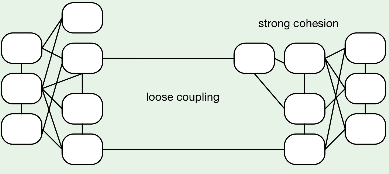
\includegraphics[width=0.3\textwidth]{images/loose_coupling}
\end{figure}
